\documentclass[output=paper]{langscibook} 

\author{Scott Grimm\affiliation{University of Rochester} and Ellise Moon\affiliation{University of Rochester} and Adam Richman\affiliation{University of Rochester}}
\title{Strongly non-countable nouns: Strategies against individuality} 

\abstract{Studies in countability have uncovered a range of ontological entities which permit counting, including natural concrete individuals, discrete events, and taxonomic subkinds.  Identifying the reasons why nominal referents may \textit{not} be counted has been less successful, however, and remains controversial. This paper examines nouns that are ``strongly non-countable”, those nouns for which combination with the plural marker, quantifiers, and nearly all other forms of determination is a vanishingly rare event. This paper develops a data set of nearly 500 such nouns, adducing their strongly non-countable status from usage over a 350 million word corpus \citep{davies2009}. Through further internet searches, we attest rare, but possible, patterns of coercion available to these nouns.  We then develop a classification of  the different notional categories that these nouns belong to. Finally, we examine broad distributional patterns and argue that these strongly non-countable nouns contrast with countable nouns as to their patterns of usage, in particular,  being less discourse-salient and less referential than their count noun counterparts. 

\keywords{countability, non-countable nouns, coercion, abstract nouns}}



%This study sheds light on properties of nominals which inhibit the ability to be counted, of which two are primary: (i) the noun’s intrinsic semantics which does not contain specifiable events or individuals (parenthood) or (ii) the noun describes a summation or collection of heterogeneous elements, thus prohibiting a stable strategy of re-identifying referents across contexts (traffic).


% \newcommand{\ipa}{\textipa}
% \newcommand{\bex}{\begin{exe}}
% \newcommand{\eex}{\end{exe}}
% \newcommand{\bxl}{\begin{xlist}}
% \newcommand{\exl}{\end{xlist}}
% \newcommand{\bi}{\begin{itemize}}
% \newcommand{\ei}{\end{itemize}}
% \newcommand{\fnc}[1]{\textrm{#1}}
% \newcommand{\bc}{\begin{center}}
% \newcommand{\ec}{\end{center}}
% %\newcommand{\posscitet}[1]{\citeauthor{#1}'s (\citeyear{#1})}
% \newcommand{\sposscitet}[1]{\citeauthor{#1}' (\citeyear{#1})}

%\newcommand{\meta}[1]{{\sc #1}}%for metalanguage discussion of terms
%\newcommand{\obl}[1]{{\itshape #1}} %introducing object language
%\newcommand{\term}[1]{{`#1'}} %introducing terms

% \DeclareMathOperator{\OU}{OU_{i}}
% \DeclareMathOperator{\KU}{KU_{w}}
% \DeclareMathOperator{\RealizeInt}{R_{i}}
% \DeclareMathOperator{\Realize}{R}
% \newcommand{\lam}[1]{$\lambda #1 $}
% \newcommand{\exis}[1]{$\exists #1 $}
% \DeclareMathOperator{\Taxon}{T_{w}}
% \newcommand{\sem}[1]{\ensuremath{\llbracket#1\rrbracket}}

\begin{document}
\SetupAffiliations{mark style=none}
\maketitle

\section{Introduction: Assessing the varieties of non-countable nouns}
%Despite the wealth of recent work on countability, it remains relatively controversial how many relevant categories of nouns can be discerned.  
When a noun has a countable interpretation, it is often intuitively clear why the countable interpretation comes about: The noun references some sort of unit which permits counting. The nature of this unit may be different depending on the noun, whole objects of the natural kind sort (\textit{dogs}) or measurement units (\textit{kilos}) to give just two examples among many, but it appears reasonably straightforward to identify that there is a unit and that that is what is being counted.

 When a noun fails to permit a countable interpretation, the situation is usually far less clear. Much research over the last two decades has gone into distinguishing two types of non-countable nouns: \textsc{substances}, those nouns traditionally considered to be ``mass" such as \textit{water} or \textit{clay}, and \textsc{aggregates}, including \textit{furniture}, the most famous example, along with other nouns such as \textit{jewelry} or \textit{mail}. The non-countability status of substances has traditionally been supported by the strong intuition that neither \textit{water} nor \textit{clay} in their primary uses make reference to individual units, more technically speaking `atoms', which would serve as a basis for quantification. %\citep{ADD-CITATIONS}.  
 In contrast, \textit{furniture} and other nouns of the aggregate type \textit{do} refer to individuals, despite their grammatical non-countability status.  Theoretical models of countability have mostly been content to account for these three types of nouns: individuals, substances and aggregates (see, for instance, \citealt{Bale2009}, \citealt{Chierchia2010}, or \citealt{Deal2016}).  Most agree that the grammatical contrasts among these noun types reflect an ontological contrast although it is a matter of controversy as to how tight the relation is.  

This paper contends that the challenge of accounting for non-countable nouns is far greater than typically assumed in the literature  and establishes some basic results on the diversity of non-countable nouns in English.\footnote{See also \citet{Allan1980} and \citet{kiss2016sense} for other larger-scale studies which help establish the diversity of countable and non-countable nouns, as well as \citet{sutton2019singular} and \citet{Sutton_Filip_2020}, which provide recent empirical work on certain domains of abstract nouns.}   We will have little to say about the different virtues or short-comings of any particular theoretical account of non-countable nouns in this paper, instead we limit ourselves to establishing empirical baselines as to what types of non-countable nouns there are and how they behave contextually and grammatically.


The structure of the paper is as follows.  In \sectref{gri-ric:sec:varieties}, we establish our methodology and, through corpus work, isolate close to 500 nouns that are rigidly non-countable or nearly always so. \sectref{gri-ric:sec:coercion} asks if these nouns \textit{ever} are counted and examines  the different patterns of coercion observed through further internet-based searches and categorizes them.  In \sectref{gri-ric:sec:notional}, we elaborate a classification of  the different notional categories that these nouns belong to, which themselves fall into four super-categories: Entities, Eventualities, Phenomena, and Abstract.  We then examine the correlation between the different notional categories and the  different types of coercion observed in \sectref{gri-ric:sec:coercion}.  \sectref{gri-ric:sec:quantitative} examines broad distributional patterns of these nouns at the level of clauses and nominal phrases, demonstrating that, on average, the non-countable nouns of our data set show behavior consistent with less discourse-salient and less referential uses.  We conclude in \sectref{gri-ric:sec:outlook}.




Our aim is that this study will facilitate the investigation of non-countability in several directions.  First, establishing, initially for English, what the lexical variation is among non-countable nouns, viz.\ what types of nouns have non-countable readings?  Answering this question   with a systematic approach will hopefully open up avenues for cross-linguistic comparison: Do the countability statuses of different notional categories co-vary across languages?  Clearly, answers to these questions will help test the predictive power of current theories: What would a theory look like that not only explains the non-countability of \textit{water} and \textit{furniture} but also of \textit{coriander}, \textit{parenthood}, \textit{fun}, or \textit{sportsmanship}?  Ultimately, this effort contributes to understanding the causal foundations of non-countability.






\section{Methodology: Discovering strongly non-countable nouns}\label{gri-ric:sec:varieties} 

%While the literature on countability has been dominated by non-countable nouns referring to substances and liquids such as \textit{sand} or \textit{water} and nouns like \textit{furniture} or \textit{jewelry}, but beyond those types of nouns, there has been little work to understand the range of non-countable nouns and the potential reasons for their resistance to being counted. 

To assess the spectrum of non-countable nouns, we extracted a large set of nouns which, based on several measures, showed the lowest degree of countability. We chose those with the lowest degree of countability in part to exclude polysemous nouns, also known as ``dual-life''  or ``flexible'' nouns, and to  minimize interference from nouns lending themselves to secondary interpretations through coercion.  In all, we assess nearly 500 nouns, a  sufficient quantity to deliver insight into potential  classes of non-countable nouns while remaining of  a manageable size.

The non-countable nouns were selected from the database described in \citet{GrimmWahlang2020}, derived from a 350 million word portion of the Corpus of Contemporary English \citep{davies2009}.  This was subsequently processed via a natural language processing (NLP) pipeline, parsing and annotating each occurrence of each noun with all relevant dependencies in which the noun stood (using Universal Dependencies from \citealt{de-marneffe-etal2014}).  This process captured a vast amount of distributional information about each noun, permitting further analytical investigation of nouns' behaviors.  (See \citealt{GrimmWahlang2020} for further details on the corpus processing and database development.)

We filtered this database to extract strongly non-countable nouns. Occurrence in bare plural was found in \citet{GrimmWahlang2020} to be the strongest predictor of countable nouns in the database, so we filtered the data most tightly on this feature, requiring a noun's  percentage of occurrences in the bare plural  to be lower than 2\% of all occurrences and, additionally, occurrence with numeric modifiers to be lower  than 20\%. We allowed for some amount of flexibility in these constraints to account for possible noise in the corpus data, due to parsing or other processing errors, as well as to not exclude rare coerced occurrences of the noun.  We allowed for more flexibility in the occurrence with numeric modifiers  since, for our purposes, there is a larger amount of noise due to how  \citet{de-marneffe-etal2014} treat numeric modifiers, since they include under numeric modifiers not only cardinal numbers and the like but also measure terms such as \textit{2 kilos} (which do not discriminate between countable and non-countable nouns).\footnote{The settings for these filters are not the only ones possible, and are proposed based on our (subjective) experiments with different percentages for both of the filters and examining the resulting sets of nouns.  These settings were felt to be optimal for permitting some level of noise or ambiguity while also narrowing down the set to truly non-countable nouns.}





 

 To select the best candidates, the data was sorted first by the lowest bare plural noun percentage (giving preference to nouns with the least noise in that category), then by lowest proper noun percentage (that is, those nouns which were very rarely, if at all, tagged as proper nouns, thereby excluding proper nouns, like \textit{William} or \textit{Cincinnati}, which would have almost no occurrences in the plural), and then highest value of overall occurrences (to preference nouns that we had the most data for).  The resulting data was further filtered to only include nouns coded as uncountable in the CELEX database \citep{CELEX} as another measure to narrow our scope. Finally, we selected only nouns for which there were greater than 200 example sentences in our data, giving us sufficient data from which to generalize. From this sorted list, we selected the top 550 nouns as the starting point for our research,  assuming that around 50 of these would ultimately be excluded due to noisiness in the data or ambiguity between multiple senses.


This list of 550 nouns was then further pared down by hand during the process of analyzing nouns for rare and contextual count examples using Google searches (see \sectref{gri-ric:sec:coercion}). A number of these searches returned established countable uses of the noun (e.g. \textit{prospects}, \textit{writings})  which led us to remove that noun from our list. In total, 26 nouns had enough count examples to be excluded from the data and 42 nouns had multiple distinct senses (some of which were highly countable), gerund uses, or appeared almost exclusively in fixed phrases (\textit{in spite of}) and so were also excluded. With the final list of 482 nouns, we built a dataset containing distributional information with the data from \citet{GrimmWahlang2020} for each noun, as well as additional data compiled from COCA example sentences. This provided us with not only summary statistics for the behavior of each noun (e.g., the percentage of occurrences with the definite article or as the subject of the verb phrase) but also lists of the unique modifiers (e.g., adjectives, case modifiers, possessive constructions) compiled from every example in our data pulled from COCA. For the comparison between the grammatical distribution of strongly non-countable nouns and countable nouns in \sectref{gri-ric:sec:quantitative}, this data set was also extended with a set of core countable nouns, grouped separately, from data in \citet{GrimmWahlang2020} (clusters 7 and 8, containing 799 count nouns).

In addition to this distributional information, our final dataset also contains data on each noun's countability as well as derivational morphology from CELEX \citep{CELEX}, hand-annotation of each noun's notional category (see \sectref{gri-ric:sec:notional}), and the possible count coercion contexts that noun was found to appear in (as discussed in \sectref{gri-ric:sec:coercion}). A separate file contains examples demonstrating each type of coercion found for each noun. We have made the final dataset and accompanying files publicly available at \url{https://quantitativesemanticslab.github.io/}.

%Structuring our data set in this way allowed us to analyze and display syntactic and morphological differences between our strongly non-countable and countable nouns, as well as between sub-groupings of nouns. %It also allowed us to compare our notional intuitions with the distribution of specific syntactic and morphological features, which we will discuss in detail in \sectref{gri-ric:sec:quantitative}.

%**NOT QUITE RIGHT** While our approach, with some post-processing, excluded polysemous nouns, further analysis, as presented in \sectref{gri-ric:sec:coercion}, indicates that the ability of even these strongly non-countable nouns to be coerced is pervasive.  

%\subsection{Generating the data set}

\section{The contexts of coercion} \label{gri-ric:sec:coercion}

While our data set contains a large number of occurrences for each noun considered (at least 200), this is not sufficient to determine if a noun which is normally non-countable \textit{ever} gets counted, and if so, upon which basis that counting is carried out.  To examine valid, albeit rare, countable examples of these nouns, we performed a battery of Google searches for each  of the 482 nouns. For each noun, we searched for occurrences with the definite article \emph{the}, plural demonstratives \emph{these} and \emph{those}, numerals \emph{two} and \emph{three}, as well as quantifiers \emph{some}, \emph{many}, and \emph{multiple}. We limited ourselves to inspecting the first five pages of results per search ($\sim$50 results per search), which in practice was sufficient to turn up any countable uses.\footnote{We ignored  a range of occurrences with plural forms that arose in uses with proper nouns, in typos, translations, non-native uses, or misuses.} 

% for plural forms or occurrence with a numeric modifier to check for any countable examples not captured in our source corpus.
\begin{sloppypar}
We collected a number of example sentences demonstrating each type of countability coercion observed with a given noun. Table \ref{gri-ric:tab:coercion} lists the different countable uses, which we will refer to as \textsc{coercion types}, observed of the 482 nouns in the data set and provides the number of nouns observed for each coercion type. While no countable examples were found for 262 of the nouns, the remaining nouns had examples that could be attributed to one or more coercion types.
\end{sloppypar}

\begin{table}
    \begin{tabular}{lr}
    \lsptoprule
        Coercion type    &  Number of nouns observed \\ 
  \midrule
 Entity Type  & 96 \\
 Event  & 67 \\ 
 Possessor  & 35 \\
 Relational & 29 \\
 Event Type  & 24 \\
 Packaging  & 8 \\
 Value & 6 \\
 Modificational & 4 \\
 Countable only in specific contexts\footnote{I.e. jargon.} & 126 \\
 Archaic\footnote{All count uses predate 1880.} & 59 \\
  No countable uses observed & 137 \\
  \lspbottomrule
\end{tabular}
    \caption{Types of countable uses of non-countable nouns. \emph{Note}: As some nouns were found to have more than one type from multiple example sentences, the ``Number of nouns observed'' column does not sum to 482.\label{gri-ric:tab:coercion}}
\end{table}


The coercion types were determined by the authors and a research assistant who separately annotated the collected examples.\footnote{This was carried out on a portion of the data for Jargon and Archaic had already been excluded.} They discussed the annotations and agreed upon a final set of labels on a small training portion of the data (150 example sentences). Then two of this group served as annotators independently annotated the remaining 377 example sentences and compared their annotations.  Inter-annotator agreement was `moderate' (Cohen's $\kappa$ = 0.56) when calculated on the entire test dataset (527 sentences). Agreement was even higher on two subsets of the data.   One subset excluded even more archaic or jargon uses and the inter-annotator agreement was `substantial' (Cohen's $\kappa$ = 0.65), and similarly for a different subset which excluded a specific error pattern from one of the annotators who over-labeled with the Packaging coercion type (Cohen's $\kappa$ = 0.66).\footnote{See full data set at \url{https://quantitativesemanticslab.github.io/}.}


Since the theoretical understanding of different types of coercions possible -- beyond the familiar contexts discussed in the literature under ``packaging'' and ``grinder''  -- is still limited, despite a growing literature which describes some of the lesser-studied countability shifts \citep{Huddleston2002,grimm2014individuating,Husic2020,ZamparelliToAppear},   we now detail with examples the different coercion types we observed for these nouns.


\begin{description}\sloppy
\item[Entity Type:] These count uses refer to multiple classifications, compositions, severities, etc.\ of the entity designated by the lexicon. As a heuristic diagnostic, \emph{type of} or a similar phrase may be felicitously added to clarify the contrast evoked.
\eanoraggedright \label{gri-ric:ex:twines}
\textbf{Twines} can differ by their material and strength, which changes how they should be used. Some \textbf{twines} are ideal for cooking since they can withstand heat and don’t impart flavor onto your food, while other \textbf{twines} are perfect for decoration or more heavy-duty use.\footnote{\url{https://www.webstaurantstore.com/guide/880/types-of-twine.html}} \z

\eanoraggedright \label{gri-ric:ex:agricultures} We now face two \textbf{agricultures}. The long-term model is exploitive and degenerative, while the new model is regenerative and more profitable.\footnote{\url{https://www.farmprogress.com/management/we-now-face-two-agricultures}} \z



\item[Event:] These count uses refer to multiple occurrences or iterations of the event designated by the noun. If the events \textit{are not} simultaneous, ordinal numerals or lexical items denoting temporal location may stand in to distinguish the events, as in  \REF{gri-ric:ex:automations}. %\todo{Can you explain/exemplify this?}
If the events \textit{are} simultaneous, other modifiers such as locations may be used to distinguish the events, as in \REF{gri-ric:ex:minings}.
\eanoraggedright \label{gri-ric:ex:automations}
The \textbf{automations} are not necessarily run at the top of the hour, and it may not be exactly one hour between executions of an automation.\\\null\hfill (Google Books) 
%\url{https://books.google.com/books?id=xyWfhzY3EI4C&pg=PA137&lpg=PA137&dq=%22the+automations%22&source=bl&ots=NoysrSY6QO&sig=ACfU3U0VxrQFazENIRgpAv9FF-zw49140A&hl=en&sa=X&ved=2ahUKEwi4lsbg0afqAhXHW80KHWM-DxUQ6AEwBXoECAwQAQ}
\z 

\eanoraggedright \label{gri-ric:ex:minings}
Most important of the \textbf{minings} were those of the Gotthard and Simplon tunnels.\hbox{}\hfill\hbox{(Google Books)}
%https://books.google.com/books?id=VHiujZyPrIAC&pg=PA67&lpg=PA67&dq=%22the+minings%22&source=bl&ots=w99xRJFZpp&sig=ACfU3U2rJk28dHBkV5xbQCPaIsTqMYUIMQ&hl=en&sa=X&ved=2ahUKEwjjn_DWqZbqAhWBGM0KHcVeCB04ChDoATACegQICRAB#v=onepage&q=%22the%20minings%22&f=false
\z


\item[Possessor:] These count uses make reference to distinct agents displaying the property, often implicitly.

\eanoraggedright \label{gri-ric:ex:sobrieties} The management team understands how individualized the recovery process is and that no two \textbf{sobrieties} look the same.\footnote{\url{https://m.yelp.ca/biz/the-district-recovery-community-huntington-beach}} \z


\item[Relational:] These count uses  arise from distinguishing multiple types in terms of their relation to, e.g., other event participants.  In example \REF{gri-ric:ex:contentments}, different types of \textit{contentment} are established with respect to the different things with which one may be content, i.e., different stimuli.

%\ea  \label{gri-ric:ex:bondage} Some of these \textbf{bondages} may include immorality, hatred, and envy. (Google Books)\z

\eanoraggedright \label{gri-ric:ex:contentments} Those \textbf{contentments} have come to include housing, healthcare, schooling and employment as well as freedom from intimidation.\footnote{\url{https://reader.exacteditions.com/issues/59737/page/10}} \z

\item[Event Type:] While countable Event uses refer to multiple, specific occurrences of the event designated by the noun, Event Type uses do not refer to specific events, but more abstractly, contrasting different types of the event in question.


\eanoraggedright \label{gri-ric:ex:violences} Again, this is not to hold equivalence between either the types of violence or particular \textbf{violences} in each category. \hfill (Google Books)\z



\item[Packaging:]  These count uses  evoke a bundling or containment of the noun's referent as a single unit, often assuming a standard measure or container. %Packaging uses may have a lexical item inserted to describe the bundling.

\eanoraggedright \label{gri-ric:ex:buttermilks}
Six quarts of milk, two \textbf{buttermilks}, two chocolates, and three pints of cream. \hfill (Google Books)
%\footnote{https://books.google.com/books?id=zl-Hbye_gL8C&pg=PT23&lpg=PT23&dq=%22two+buttermilks%22&source=bl&ots=53-lvMz3cV&sig=ACfU3U0NWhwujseQ8_mNLlaglzBWjNg5gw&hl=en&sa=X&ved=2ahUKEwiOivm_mKvqAhUFBs0KHXiPCDMQ6AEwA3oECAkQAQ}
\z


\item[Value:] These count uses refer to varying levels or numerical values of a scale associated, perhaps implicitly, with the noun. This use differs from Entity Type coercions as this relies on a value or degree. Explicit values may be added to distinguish between the singular units.

\eanoraggedright \label{gri-ric:ex:latitudes} Low \textbf{latitudes} are those locations found between the Equator (0 degrees N/S) and 30 degrees N/S. The middle \textbf{latitudes} are found between 30 degrees N/S and 60 degrees N/S. And the high \textbf{latitudes} are found between 60 degrees N/S and the poles (90 degrees N/S). \footnote{\url{https://www.shsu.edu/~dl_www/bkonline/131online/f02latitude/02index.htm}} \z

\eanoraggedright \label{gri-ric:ex:moistures} Barley was germinated in soils of two \textbf{moistures} (40 and 50 per cent). \hfill (Google Books) \z


\item[Modificational:] These count uses are of (typically) adjectives, where the head noun is absent and the modifier or distinguishing property is actually what bears the plural morphology.

\eanoraggedright \label{gri-ric:ex:vanillas} If there really were 6 vanilla and 6 peanut butter candies in the box, what is the probability that you would have picked three \textbf{vanillas} in a row?\footnote{\url{https://www.slader.com/discussion/question/someone-hands-you-a-box-of-a-dozen-chocolate-covered-candies-telling-you-that-half-are-vanilla-cre-2/}} \z


\item[Jargon:] These are count uses that  occur only within specific contexts, primarily technical jargon. The example in \REF{gri-ric:ex:oxygens} is a commonly found example of jargon occurring in chemistry and physics contexts that describe atoms and molecules.

\eanoraggedright \label{gri-ric:ex:oxygens}
However, at the oxygens bridging two \textbf{aluminums}, oxygens were swapped only about once every 13 hours.\footnote{\url{https://www.ucdavis.edu/news/oxygen-swapping-offers-clues-toxics-management/}}
\z 

%\ea \label{gri-ric:ex:atoms}
%However, at the oxygens bridging two \textbf{aluminum \emph{atom}s}, oxygens were swapped only about once every 13 hours.
%\z


\item[Archaic:] These count uses occur only in poetic uses or examples predating 1880, and current countable uses are not found outside of these contexts. 
\eanoraggedright 
The capytle doth shew of the \textbf{fortitudes} of the planetes.\\\hbox{}\hfill\hbox{(Google Books)}
%\url{https://books.google.com/books?id=DQZVAAAAcAAJ&pg=PA23&lpg=PA23&dq=%22the+fortitudes%22&source=bl&ots=RIiqLE8V2C&sig=ACfU3U0g6dzYeLUVMCMQJATS4xLaKmjlIQ&hl=en&sa=X&ved=2ahUKEwiNp8ff6JrqAhWUG80KHaU3BGoQ6AEwD3oECAsQAQ#v=onepage&q=%22the%20fortitudes%22&f=false}
\z


\item[No countable uses observed:]  These nouns had no occurrences of count uses. 

\end{description}



In summary, this data set leads us to observe a wide range of possible shifts  from non-countable to countable interpretations, many of which have been little explored at this point.  %Even heavily-discussed forms of coercion, such as packaging, appear in a different guise here, since often, despite a clear use of packaging, there is no ``standard portion'' that can be assumed for the noun under discussion, as is the case for `oxygens' in example \REF{gri-ric:ex:oxygens}. \todo{isn't it individual atoms? Also isn't the noun in (1) \textit{aluminium}? I'd say we could find a clearer example if we make this point here -E} \todo{go through all the count labels again, redo them} 
For Type coercions, while there is some discussion and even controversy about (the lack of) subtype coercions (see \citealt{grimm2016artifact} and \citealt{sutton2016counting} and references therein), it has primarily revolved around nouns describing liquids or substances (\textit{wines}) and artifactual aggregates lacking subtype readings (\textit{furniture}), yet there are many other domains to check to see how type coercion is effected, as exemplified  in \REF{gri-ric:ex:agricultures}.   The interpretational shifts we list under Event and Possessor have to date only received brief treatments \citep{grimm2014individuating, ZamparelliToAppear, Husic2020} and similarly for Relational \citep{grimm2014individuating} (although a more sophisticated treatment has begun to be developed for informational nouns in the line of work of \citealt{sutton2019singular} and \citealt{Sutton_Filip_2020}), while the observation of Value-based and Modificational count shifts is novel to the best of our knowledge.  Again, it is possible that this classification stands in need of revision and, for instance, Relation or Value could be grouped under Type if understood more broadly, but we have erred on the side of being more explicit to bring out some of more unusual cases of coercion observed.  A related issue is if all of the examples examined are truly cases of coercion as opposed to polysemy -- again we have erred on the side of inclusion as coercion when a plausible case can be made.

\section{The notional varieties of strongly non-countable nouns}\label{gri-ric:sec:notional}  


A major theme of countability research is the relation between contrastive grammatical countability classes and corresponding contrasts, or lack thereof, of notional, or ontological, types of the corresponding referents of the grammatical classes.  %In fact, most semantic theories of the count/mass distinction are grounded in reference, positing different referential types as being responsible for the differing countability behavior of nouns.   
As mentioned, several authors propose that the referential types of individuals, aggregates, and substances are those that are responsible for countability contrasts \citep{Bale2009,Chierchia2010,Deal2016}. It is therefore critical to examine the relation between the strongly non-countable nouns and their corresponding notional types.   The different notional types brought forth by the strongly non-countable data demonstrate that those referential types may be necessary to account for the grammatical behavior related to countability, but those three types are far from sufficient.  Instead, we observed rich variation in the notional types that correspond to strongly non-countable nouns, transcending the contrasts typically  posited to explain grammatical countability patterns, as in those between, e.g., substances vs.~individuals vs.~aggregates or events vs.~states.  




\subsection{Notional categories of strongly non-countable nouns}

This section puts forth a classification of the 482 nouns into 27 separate ``notional'' categories, such as \textsc{liquids} or \textsc{disease}.    While the categorization presented here no doubt reflects some core aspects of the nouns' meaning, we hasten to emphasize that this classification is preliminary -- nearly all of these nouns have never been systematically analyzed and we do not pretend to have been able to fully analyze them here.  That said, even this initial categorization establishes  that the range of notional noun types which show strongly non-countable behavior is far greater than one would suppose from the discussions in the literature.  %Further, although the categories presented here often differ in their grammatical properties, it is not clear 



Table \ref{gri-ric:tab:1:Notional} (page \pageref{gri-ric:tab:1:Notional}) displays the categorization.  The 27 categories are broadly grouped into four super-categories: Entities, Eventualities, Phenomena, and Abstract.  These are organized in terms of the apparent ontological commitments of the nominal descriptions falling under each category: Entities includes nouns describing entities rooted in physical existence (``concrete entities''); Eventualities includes those entities rooted in a temporal dimension, here using the term ``eventualities'' in the sense of \citet{Bach1986} for both events and states; Phenomena~-- such as diseases or natural forces -- while having a connection to the physical world are more abstract than the concrete objects found in Entities; and Abstract contains nouns that are, at least on their primary reading, detached from the physical world, comprised of nouns describing, e.g., atemporal, non-physical qualities (\textit{cleanliness}) or domains of knowledge (\textit{geology}).     In the following, we discuss the different categories and their nouns and note their particularities against the background of the expectations from the countability literature.%, **FIX**in so doing we make some preliminary observations of the sources of non-countability for these nouns.

\begin{sloppypar}
These proposed categories can also often be distinguished via contrasting grammatical properties, often those related to the argument structure considerations.  For instance, unlike pure substances, the \textsc{by-products} category contains nouns that allow a \textit{from} argument which specifies from where the substance originated (\textit{refuse from the facility}).  Similarly, \textsc{mental states} differ from \textsc{general states} in that the former, such as \textit{awe} require a participant who is mentally engaged in the event.  While these grammatical contrasts have informed our categorization, we only discuss them in passing as they do not directly map onto countability contrasts.
\end{sloppypar}


\begin{table}
\caption{Notional classes of non-countable nouns}
\label{gri-ric:tab:1:Notional}
 \begin{tabular}{ll} 
  \lsptoprule
    {Category}    &{Examples}\\ 
  \midrule
  \multicolumn{2}{l}{Entities (108)}\\  \midrule
%   \multirow{11}{*}{\STAB{\rotatebox[origin=c]{270}{Entities}}}\\
%   &\multirow{11}{*}{ (108)}
    aggregates (27)  &   footwear, furniture, glitter, traffic \\
  by-products (10)  &  garbage, rubble, sawdust, soot \\
  chemicals \& elements (20) & ammonia, glucose titanium, uranium  \\
  drugs (7)  &   cocaine, morphine, nicotine \\
  %&&elements (12)  &  calcium, chlorine,  \\
  meat (3)  &  pork, poultry, venison \\	
  grains/flours (4) &  bran, flax, oatmeal   \\
  herbs and spices (11) &   cumin, nutmeg, paprika, parsley \\
  materials (11) &   carpeting, denim, plywood \\ 
  liquids (11)  &  bile, buttermilk, oil, rainwater \\ 
  natural substances (4) & dirt, driftwood, flesh, quartz \\\midrule
  \multicolumn{2}{l}{{Eventualities (109)}} \\\midrule
    % \multirow{7}{*}{\STAB{\rotatebox[origin=c]{269}{Eventualities}}} 
%   &\multirow{7}{*}{ (109)}
   events  (8) &   atonement, bribery,  legalization \\
  multi-participant events	 (6) & acclaim, applause, bloodshed, gunfire \\
  coming-into-/going-out-of-exist.~(13) & abolition, emergence, eradication\\
  mental states	(28)  & awe, bewilderment, remorse, unease \\
  general states (17)& illiteracy, prosperity, puberty    \\
  activities (25) & banking, espionage, gardening \\
  gradual/repeated processes (12) & conservation, enforcement \\\midrule  
 \multicolumn{2}{l}{{Phenomena (21)}}\\\midrule
%   \multirow{2}{*}{\STAB{\rotatebox[origin=c]{270}{Phenomena}}}
%   &\multirow{3}{*}{ (21)} 
   diseases (6) &   arthritis, flu, hepatitis, herpes \\	
  disorders (7)  &  alcoholism, amnesia, anorexia \\
  natural force (8)&   antimatter, electricity,  momentum \\
%   \ &&&\\
\midrule  
 \multicolumn{2}{l}{{Abstract (212)}}\\
  \midrule
%   \multirow{5}{*}{\STAB{\rotatebox[origin=c]{270}{Abstract}} } 
%   &\multirow{5}{*}{ (212)}
    domains  (16) &  agriculture, geology, journalism \\
  social ideas (27)  &   communism,  conservatism \\
   general quality (52) & cleanliness, permanence, resiliency \\
  human quality (55) & cynicism, sportsmanship, stardom   \\
  asymmetric relations (25) &  abstinence,  paucity, precedence \\
  symmetric relations (11) &  coexistence, companionship, peace\\
  sports (16)&  archery, golf, soccer \\
  location/time (10) & airspace, dawn, latitude  \\\midrule
  unclassified (32)  & fun, haste,  parenthood \\
  \lspbottomrule
 \end{tabular}
\end{table}





\subsubsection{Entities} The Entities super-category includes some representatives of ``classic'' non-count\-able noun types, such as \textsc{substances} (\textit{dirt}), \textsc{materials} (\textit{asphalt, hemp, latex}), \textsc{grains and flours} (\textit{bran,
cornstarch, flax}), and  \textsc{liquids} (\textit{booze, kerosene, oil}).  Although these notional categories are the most typical ones used to exemplify non-countable nouns (e.g.\ \textit{water}, a liquid) in our data, these categories are somewhat sparsely populated compared to the number of other categories (e.g., mental state nouns).  No doubt this results from the high number of nouns in these categories which are ``dual-life'' nouns, that is, nouns which also manifest a countable use and thus were excluded from our set of strongly non-countable nouns. At the same time, other instances of liquids and substances do arise, namely those that have been processed or manufactured, falling under the  categories of \textsc{chemicals \& elements} and \textsc{drugs}.   

Better represented are \textsc{aggregate} nouns, for which nearly all the examples from the literature are found in our data set (\textit{footwear, furniture,  luggage, silverware}) along with nouns which have some claim to ``aggregate'' status, even if most likely possessing some different characteristics than \textit{furniture}, such as  \textit{bedding}, \textit{homework}, \textit{merchandise}, \textit{paperwork}, \textit{parking}, \textit{traffic}, \textit{weaponry},  and \textit{wildlife}.  Thus, our methodology is able to replicate the observation made at several points in the literature that aggregate nouns like \textit{furniture} are less flexible and therefore more strongly non-countable than typical substance or liquid nouns.%**CITE**







\begin{sloppypar}
The  category \textsc{by-products} collects nouns that either  designate materials which result from some prior activity  (\textit{rubble}, \textit{sawdust}, \textit{sewage}, \textit{smoke}, \textit{soot}) or designate collections of entities or materials deemed worthless (\textit{garbage}, \textit{refuse},  \textit{trash}, \textit{filth}). While the cause for the first group's non-countability status may be similar to that of materials or aggregates, for nouns such as \textit{trash} the seeming cause of non-countability is more indirect:  Even if a use of \textit{trash} designates entities that would otherwise be countable individuals, designating (and evaluating) them with the nominal description \textit{trash} avoids identifying or individuating elements.
\end{sloppypar}

Food terms such as \textit{chicken} are well-known as ``dual-life'' nouns, but the nouns of the  \textsc{meats} category here are those that describe classes of meat (\textit{poultry, pork, venison}) for which reference to the animal is named separately.  While \textit{chicken} is often used as an example of a noun with both a count and non-count use to exemplify the claim that many nouns in the lexicon are ``flexible'' nouns \citep[e.g.][241]{Bale2009}, this is not to be taken for granted, since, for instance, \textit{pork} and \textit{pig} (or \textit{mutton} and \textit{sheep}) are not ``flexible'', that is, do not, in typical circumstances, display both a count and non-count use.  This is clearly due to the fact that the reference to the animal and the meat are accomplished by two distinct nouns, whereas in the case of  \textit{chicken}, a single noun lexicalizes both types of referents.


%and no doubt a more complete sample of nouns would include other terms such as \textit{mutton}. 


\textsc{herbs and spices}, such as \textit{coriander}, \textit{cumin}, \textit{fennel}, \textit{incense}, and \textit{nutmeg} provide another interesting puzzle.  In their physical form, many members of this class (e.g.\ a parsley plant or sprig, or a fennel bulb) are just as easy to individuate as many other small plants or bulbs which are described by countable  nouns in English (\textit{dandelion, onion}), as well as countable nouns which are similarly able to divide their reference, such as \textit{twig} or \textit{branch}.  Yet, it is presumably their use, typically as processed bits or powders, that accounts for their strongly non-countable behavior \citep{Wierzbicka1988}.

In sum, the now-common notional contrast between individual, aggregate and substance nouns is not sufficient to explain the variety of types of non-countable nouns observed even in the domain of physical entities: Evaluativity, interaction/use, and lexical contrast all may play a role in why a given noun may be (non-)countable.

\subsubsection{Eventualities} The Eventualities super-category contains nominal forms designating various events, activities, processes or states.  As one might expect from previous work linking countability and aktionsart (see \citealt{Mourelatos1978, grimm2014individuating} and references therein), the non-countable nouns in this category are imbalanced among types of eventualities. More nouns refer to activities, processes or states than to events and, further, the strongly non-countable nouns that do refer to events have very particular semantics.

\begin{sloppypar}
\textsc{multi-participant events} enforce  reference to multiple individuals or events, thus \textit{applause} normally comprises clapping from more than one member of an audience, and \textit{bloodshed} is used to describe the killing or wounding of multiple people.\footnote{Some lexicographical resources note the multiple-participant facet of \textit{bloodshed}'s meaning, as in the definition from the Oxford lexicography website \url{lexico.com}: ``The killing or wounding of people, typically on a large scale during a conflict.''}  Similarly, \textit{centralization} requires bringing multiple elements together  while  
\textit{dissemination} requires distributing multiple elements in multiple locations.  The intrinsic plurality in these nominal descriptions most likely inhibits the use of a plural form.\footnote{An anonymous reviewer suggests that this class could constitute a morphologically singular counterpart to pluralia tantum nouns like \textit{scissors} or \textit{entrails}, which have been argued to be lexically plural \citep{Acquaviva2008}, differing in that the lexical plurality is not overtly marked.}
\end{sloppypar}



\begin{sloppypar}
The category of \textsc{coming-into-/going-out-of-existence} contains nouns which describe the beginning or the end or demise of an entity, which typically is an argument of the noun, such as \textit{abolition}, \textit{emergence}, \textit{eradication}, \textit{incineration}, or \textit{regeneration}.  Thus, \textit{eradication} designates the end of some entity's or set of entities' existence, as in \textit{the eradication of smallpox}, while \textit{emergence} is the beginning of the existence of some entity or the appearance at a location.  While these eventualities designate precise points in time where the entity in question passes into or out of existence, the grounds for canonical non-countability would appear to stem from the uniqueness of the events, as entities do not typically pass into or out of existence more than once.%\footnote{FINALIZE See also remarks in \citet{grimmmcnally2013} about \textit{destruction}.} SAY MORE?
\end{sloppypar}


The category of \textsc{events} contains a rather miscellaneous set of eventive nouns which do not fit into the categories discussed above.  Those such as  \textit{atonement} or \textit{reclamation} would also appear to be rather unique occurrences and as such resist pluralization. 


The remaining categories in the Eventuality super-category are the more expected non-countable eventualities: \textsc{activities}, \textsc{gradual/repeated processes} and \textsc{states}. We distinguish two types of states.  In addition to \textsc{mental states}, which are often cited as non-countable nouns, we include \textsc{general states} (\textit{mayhem}, \textit{poverty}, \textit{unemployment}), by which we indicate nouns that refer to a general situation, equally able to be predicated of individuals and groups, and unlike the category of \textsc{general quality}, are straightforwardly compatible with temporal localization.   Many of these nouns manifest what has been termed in \citet{grimm2016crime} a ``non-particularized use,'' that is, the nouns refer to instances of, e.g., \textit{poverty}, but without making any claims to these instances being spatio-temporally located or being of a particular number.





%take stock of notional categories

%What types of nouns are there?\\
%-Discuss intuitive classification

\subsubsection{Phenomena} These nouns lack reference to any specific temporal or spatial location, the vagueness and unbounded nature of which is most likely the cause of their non-count\-abil\-ity. For instance, \textsc{diseases} includes nouns which have meanings charged with  physical and temporal aspects, e.g., \textit{smallpox} or \textit{tuberculosis} have physical causes and manifestations, but these are not the same as nouns which describe a (potentially) bounded physical entity, like \textit{table}.   Similar observations apply to  \textsc{disorders}, such as \textit{autism} or \textit{vertigo}, which are related to events, but cannot be reduced to particular events or states, as well as to \textsc{natural forces}, such as \textit{magnetism} or \textit{sunshine}.  


%Contrast with aggregates and liquids, which both can be quantified, or in the case of aggregates, unitized, this doesn't seem possible. grain of rice, bowl of rice, cup of water, bottle of oil, etc.




%Is there something vague about \textit{baseball} or \textit{chess}?



\subsubsection{Abstract} The nouns in \textsc{abstract} are those which are not necessarily interpreted as connected to spatial or temporal dimensions.  \textsc{domains of knowledge} (\textit{forestry}, \textit{psychoanalysis}, \textit{voodoo}) or \textsc{social ideas}  (\textit{federalism}, \textit{materialism}) describe bodies of knowledge, ideas or cultural practices which are not embodied by one particular act or event.  Qualities, both \textsc{human qualities} (\textit{chastity}, \textit{foolishness}) and \textsc{general qualities} (\textit{health}, \textit{toughness}), may be exemplified by acts or events, but are not co-extensional with those events.  That is, the meaning of \textit{chastity} or \textit{foolishness} is not equivalent to the set of chaste or foolish acts.  Nouns which designate relations are found in this class, too.  These are distinct from nouns most often discussed under ``relational nouns'' such as \textit{brother} or \textit{neighbor}, which designate an entity in terms of the relation it stands in with respect to another entity.  The nouns, whether in the \textsc{symmetric relations} (\textit{accordance}, \textit{relatedness}) or \textsc{asymmetric relations} (\textit{governance}, \textit{subordination}) category, designate the relation itself.  

The nouns in the category of \textsc{location/time} describe or reference some aspect of spatial or temporal experience, as in \textit{horseback},  \textit{midair}, or \textit{sundown}, but again cannot be reduced to a specific location or event.  The category of \textsc{sports} too shares the aspect of at once having physical and temporal aspects while also transcending them.  


\subsubsection{Unclassified}  The inclusion of this category  reinforces a point made at the beginning of this section, that this classification is incomplete and many unresolved issues remain.  This varied group  includes nouns such as \textit{postage}, \textit{slang}, \textit{eyesight}, and \textit{firepower}, which fit poorly in any of the categories discussed so far.  No doubt a larger sample would help to establish even more fine-grained categories in which these nouns could be located.  Some interesting cases are still worth pointing out.  

\begin{sloppypar}
\textit{Manslaughter} appears to be rigidly non-countable, which is odd if one takes it to be analogous to, for instance, \textit{murder}; however, the observed uses of \textit{manslaughter} do not appear to be directly referencing acts or events, but rather offer a classification of acts or events as falling under manslaughter or not -- that is, the noun provides a second-order property, a property of properties. In a similar vein, the nouns \textit{conduct} or \textit{haste} do not refer an event itself, but serve as a secondary predication over an event, referring to the manner in which an event or set of events was carried out.
\end{sloppypar}


Another interesting case is the small group of nouns derived by \textit{-hood}, including \textit{fatherhood}, \textit{motherhood}, and \textit{parenthood}.\footnote{\textit{Womanhood} is also included in this group, although it differs semantically from those derived from a relational noun.  Derivations with \textit{-hood} are not semantically transparent, as the countable nouns \textit{childhood}, which is temporally grounded, or \textit{neighborhood}, which is spatially grounded, attest.}  Here \textit{-hood} combines with a relational noun to derive some more abstract quality or property associated with participating in that relation.  These nouns do not appear to be stative, as evidenced by their infelicitous combination with temporal modifiers (\textit{his homelessness}/?\textit{fatherhood lasted two years}), nor do they straightforwardly fit with human qualities (\textit{composure}), which depict a quality that humans can possess or not, nor with general qualities (\textit{cleanliness}), which characterize a situation. % **FIX FINAL REMARK**


%\subsection{Interim Discussion}


In sum, the wide variation in different notional categories of non-countable nouns vividly demonstrates the challenge awaiting theories of (non-)countability.  It is unlikely that there is a single, monolithic source of non-countability for which the semantics of \textit{glitter}, \textit{homelessness} and \textit{archery} interact in the same way. To the contrary, it appears that many of the principles by which something is deemed non-countable, in English and across languages, have yet to be fully understood.     %Some of the proposed sources of non-countability,  such as  vagueness as to how much is a sufficent quantity to ``count'' as an instance or unit \citep{Chierchia2010b}, or  or that parts may overlap \citep{Landman2011}, face clear challenges in being extended across this data set.




%Vagueness: If there is no clear minimal quantity of N that counts as N (in a context), then there are no clear minimal parts of N to count.

%Overlap: The overlap of individual entities (things that count as one) is proposed as the source of the mass/count distinction in Landman (2011).


%All of these approaches are based in a search for some sort of minimal spatiotemporal   individuals

%What's wrong with that?  







\subsection{Notional types and coercion types}

We now turn to examine if correspondences can be found between the notional categories of nouns laid out in this section and the coercion types discussed in \sectref{gri-ric:sec:coercion}.  Figure \ref{gri-ric:fig:heatmap} presents a heatmap that maps the number of nouns in each notional category manifesting each type of coercion shift.  Several trends are visible upon inspecting this visualization of the data.  First, as one would expect, Packaging and Event coercions are effectively in complementary distribution, with Packaging being found among nouns of the Entities super-category and Event being found across the rest of the notional super-categories.  Second, Type coercions are robustly found across the different super-categories, although are unobserved for some of the categories, such as \textsc{aggregates}, \textsc{elements}, or \textsc{location/time}.   The Jargon and Archaic coercions are primarily found with the more eventive and abstract nouns.  The None column, which tracks the number of nouns for which no coercions were observed, shows that across the different categories there are almost always some nouns which are rigidly non-countable, while certain notional categories, such as \textsc{sports} or \textsc{natural substances}, appear to be mostly comprised of rigidly non-countable nouns.



\begin{figure}
%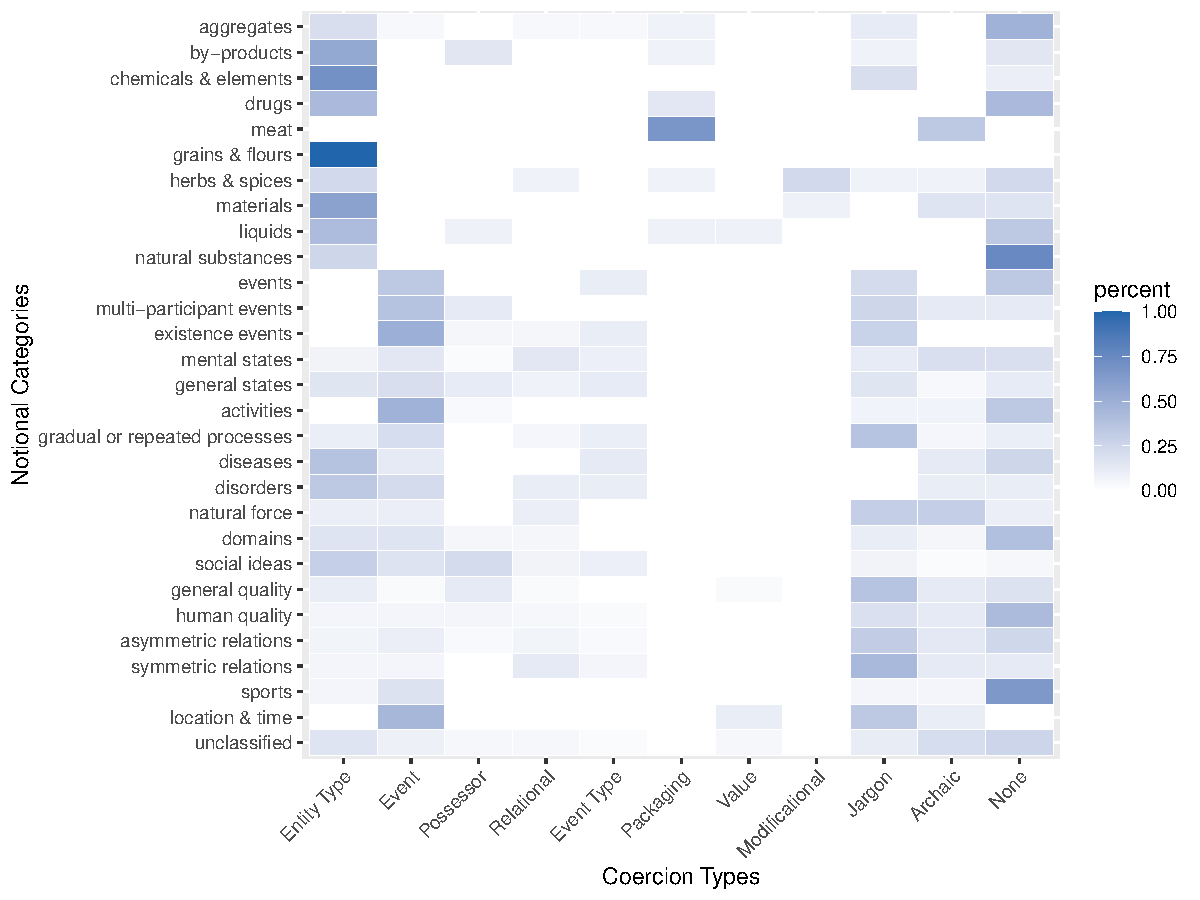
\includegraphics[width=\linewidth]{coercions-heatmap-final.pdf}
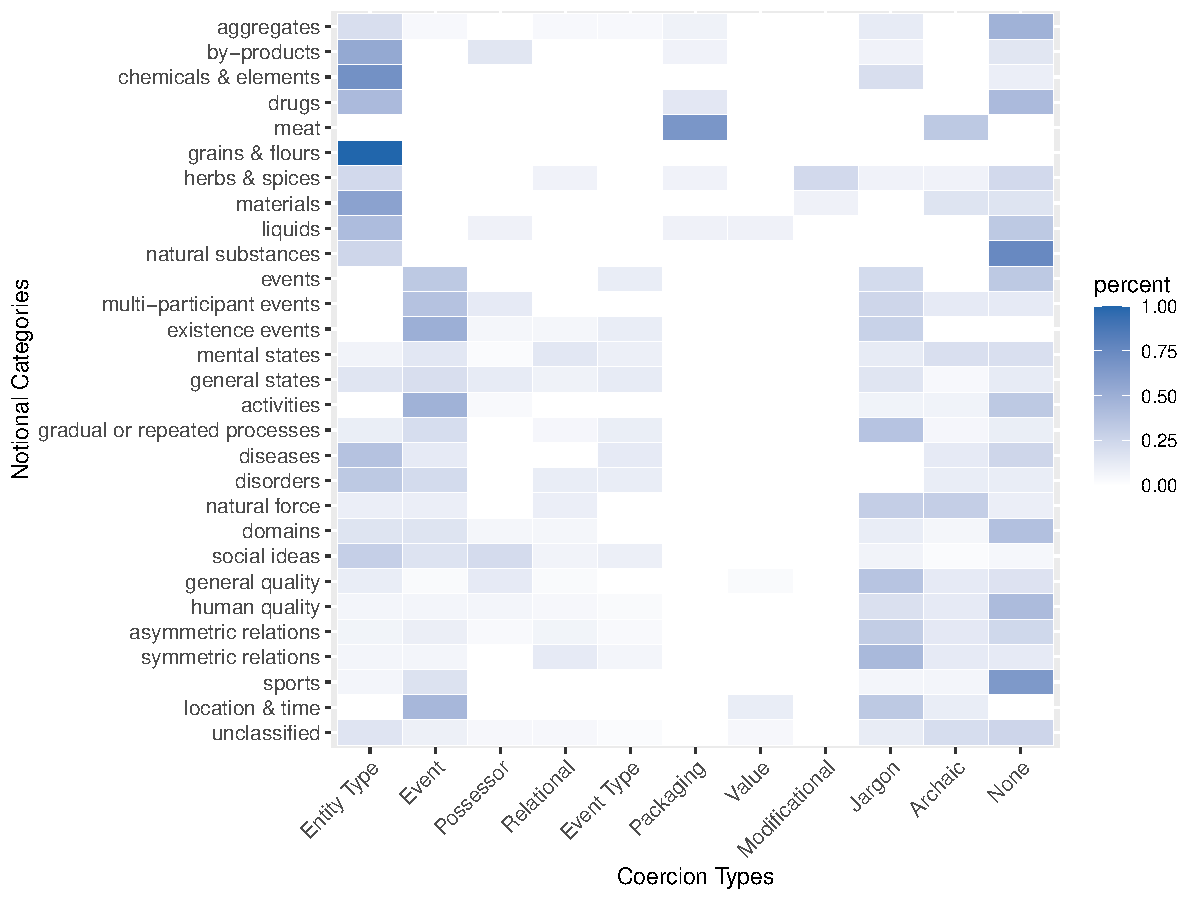
\includegraphics[width=\linewidth]{figures/Rplot03.pdf}
\caption{Heatmap showing the proportion of observed coercions in each coercion type for each  notional category}
    \label{gri-ric:fig:heatmap}
\end{figure}


A major effort for  future research is to understand which types of nominals allow which types of coercions.  We expect that contributing this explicit data set of coercions will help systematize this effort.






\section{Variation in grammatical behavior of strongly non-countable nouns}\label{gri-ric:sec:quantitative}\largerpage[-2]

This section investigates the general distributional characteristics of these nouns, beyond those solely concerned with countability.  We ask if it is possible to detect any broad scale contrasts in grammatical environments between these strongly non-countable nouns  and a group of ``standard'' countable nouns and hypothesize that these sets of nouns which already differ in countability status will also differ in two other aspects of their grammatical distribution.  First, we expect them to differ in their propensity for occurrence in different grammatical positions, i.e.\ if they are more frequently governed by verbs or prepositions and what position they have in those structures, e.g.\ verbal subject or object. Measuring the nouns' distribution in clausal position, e.g., use as subject, serves as a proxy for understanding their typical discourse salience (see \citealt{kaiser2006effects} and references therein): Verbal subjects tend to be more salient in the discourse as a whole than nouns occurring in the object position, and similarly for nouns occurring as a nominal head modified by a prepositional construction (\textit{the \textbf{ire} of parents}) as opposed to being in the complement of a preposition (\textit{the ire of \textbf{parents}}).  Second, we measure the ``referential weight'' of the nouns' uses, tracking the amount of determination, especially definite determiner usage, the noun manifests across its occurrences.  We expect countable nouns to have a higher proportion of referential (definite) uses and we use the occurrence of the definite determiner as a proxy for referential uses (while noting that this is clearly a simplification, given the complexity of the uses of the definite determiner, see \citealt{lyons1999definiteness} i.a.).  For countable nouns, on the whole, we expect more occurrences with the definite determiner and in salient argument positions (\textit{The \textbf{vase} is on the table.}) while strongly non-countable nouns will occur less often with definite determiners and in non-argument positions (\textit{The stoppages of work could not be justified by the standards of arbitral \textbf{jurisprudence}.})

Together, if validated, these hypotheses would indicate that countable nouns tend toward greater discourse salient and referential uses while strongly non-countable nouns, and perhaps non-countable nouns more generally, have fewer discourse salient and referential uses.  This is intuitively plausible insomuch as countable nouns describe entities for which it is useful to regularly pick out, or individuate, the referents.  To explore these hypotheses, we expanded our data set to include countable nouns with which we could contrast the 482 non-countable nouns.  We selected the Core Countable nouns of \citet{GrimmWahlang2020}, a set of 799 nouns identified through a clustering experiment based on distributional properties shown to be predictive of countability status.\footnote{These properties were occurrence in the bare Plural, the bare singular, and with ``unit'', ``fuzzy'' and ``other'' denumerators.  See \citet{GrimmWahlang2020} for further discussion.}

\begin{figure}
    \centering
    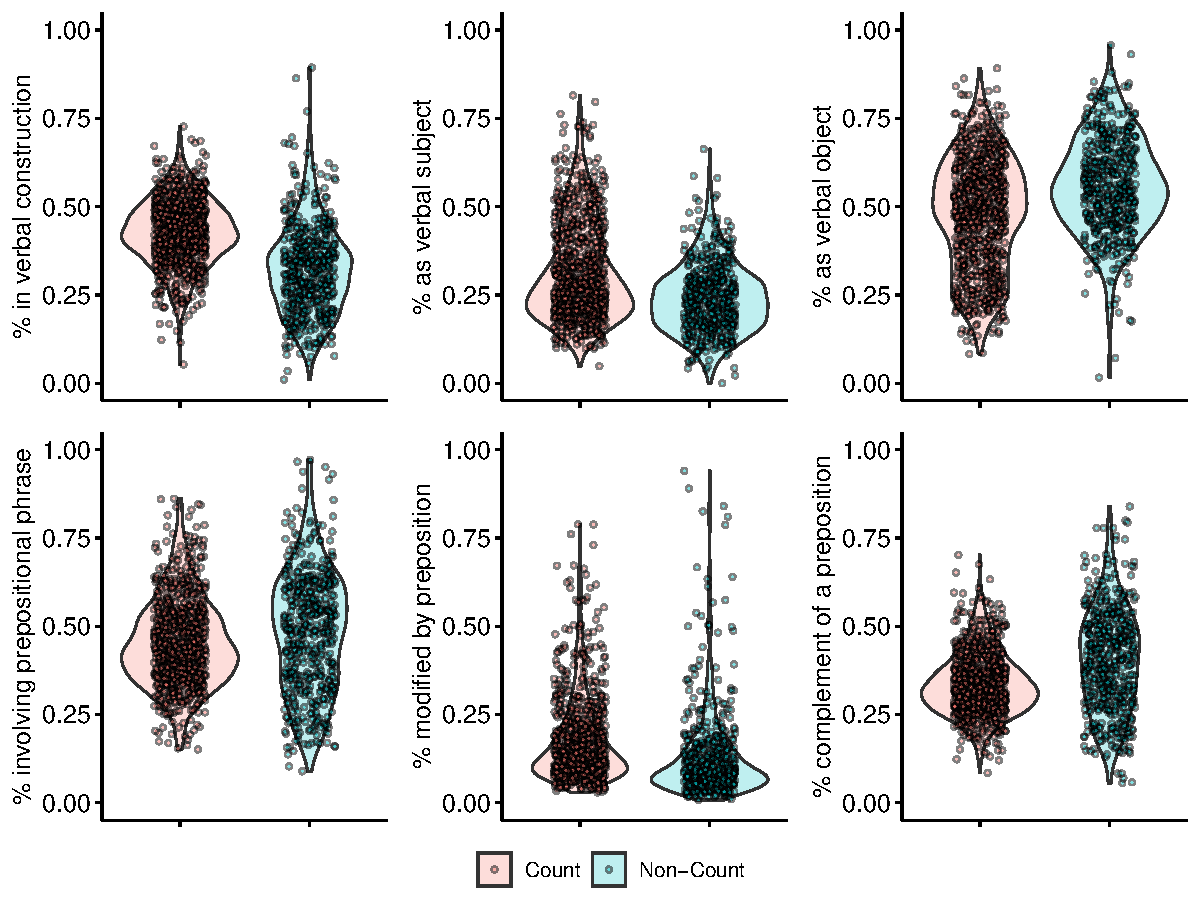
\includegraphics[width = \linewidth]{distribution-plot.pdf}
    \caption{Comparison of distributional properties of non-count and count nouns: Percentage of occurrence of each noun in  each environment}
    \label{gri-ric:fig:distribution}
\end{figure}

Figure \ref{gri-ric:fig:distribution} presents plots displaying the distribution of the grammatical positions of the countable and non-countable nouns examined.  The violin plots include each noun as an individual point and the probability density of the distribution of the sample showing the general distributional trends. The upper half of Figure \ref{gri-ric:fig:distribution} shows in the leftmost panel the nouns' occurrence in verbal constructions generally and then the proportion of a noun's verbal occurrences  as verbal subject and as object.  The lower half shows their occurrence with prepositions generally, and then, relative to the total number of prepositional occurrences, the proportion as nominal head modified by a preposition and the proportion as complement of a preposition.  As can be seen, countable nouns have a greater propensity to be in verbal constructions and to be the subject of those constructions more often than non-countable nouns do, and conversely, non-countable nouns have a greater tendency to be in object position.\footnote{All significance tests were carried out using simple $t$-tests, and all result reported as ``significant'' are of $p<0.001$. For comparisons between the distributions of singular and plural occurrences of nouns, paired t-tests were used. See further details in the data and code repository.}
%\footnote{\% non-bare: Count.SG \%, Count.PL \% Non-Count \%; \% with determiner: Count.SG \%, Count.PL \% Non-Count \%; \% with verbal subjects: Count.SG \%, Count.PL \% Non-Count \%; \% with verbal objects: Count.SG \%, Count.PL \% Non-Count \%; \% in complement of preposition: Count.SG \%, Count.PL \% Non-Count \%; \% modified by preposition: Count.SG \%, Count.PL \% Non-Count \%} %\todo{add stats} 





\begin{sloppypar}
The behaviors of the different types of nouns in prepositional phrases is more variable, especially for non-countable nouns: Non-countable nouns have a greater propensity to occur generally in prepositional phrases and to occur in the complement of  prepositional phrases than countable nouns do, but what is most striking is the far greater variability among non-countable nouns than among countable nouns.  Countable nouns can be seen to vary from approximately 25\%--75\% of occurrence in prepositional phrases with a mean tendency of  45.4\%.  Non-countable nouns range from hardly ever occurring in prepositional phrases (\textit{parking, bowling}) to nearly always (\textit{entirety, lack, emergence}), and the central tendency, at 47.7\%, is far less pronounced. %\todo{add measure of variance}  
The same contrast occurs in measuring occurrence in prepositional complement positions, with some non-countable nouns  hardly ever occurring as a complement to a preposition (\textit{shopping, gripe}) and some nearly always doing so (\textit{manslaughter, colonialism, disgust}). The rate of occurrence as the head of the prepositional phrase is similar for countable and non-countable nouns, although less frequent for non-countable nouns.
\end{sloppypar}



\begin{figure}
    \centering
    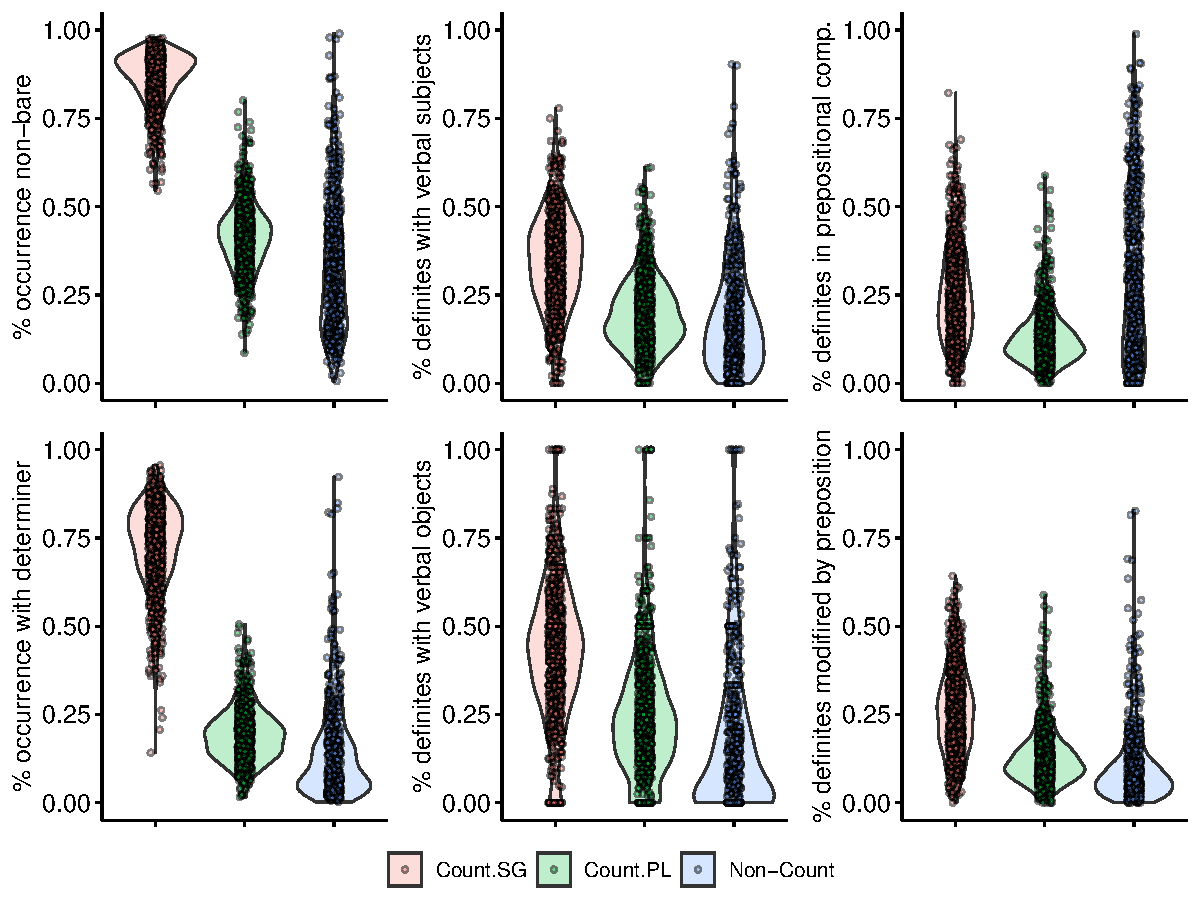
\includegraphics[width = \linewidth]{determiner-plot-final.pdf}
    \caption{Comparison of determiner distributions of non-count and count nouns: Percentage of occurrence of each noun in  each environment}
    \label{gri-ric:fig:referentialWeight}
\end{figure}




Figure \ref{gri-ric:fig:referentialWeight} presents violin plots which display the distributional traits hypothesized to correspond to the different degree of determination and referential uses among countable and non-countable nouns. For this study,  we consider the singular and plural occurrences of nouns separately, since their ability to occur without determiners differs: Plural nouns, like non-countable nouns may be bare (that is, have a ``null determiner''), while this is disallowed for countable nouns.\largerpage


The plots in the left panels display coarse-grained information about determination patterns. The upper-left panel shows the percentage of nouns' occurrences \textit{not} as bare nouns, that is, occurrences that lack any sort of quantifiers, determiners or modifiers.  The lower-left panel displays the proportion of determiners found with a given noun. Here we observe a trend that holds across all the plots. There is an ordering among the mean proportion of determination for the different groups:  Singular count nouns have the highest proportion of determiner or non-bare use, plural count nouns next highest and non-count nouns lowest.   In the upper-left panel, non-countable nouns display  a high degree of variation as to whether they occur bare, with some exclusively occurring bare (\textit{peacetime, photosynthesis}) and some most always occurring with some sort of determination or modification (\textit{fondness, nakedness, woodwork}). In contrast, countable nouns are more tightly grouped for singular and plural occurrences, with a substantial proportion of plural uses occurring bare, no doubt largely due to generic uses.   %The upper-right and lower-left panels show that non-countable nouns do have lower rates of adjectival modification and occurrence with determiners, respectively.    









The four middle and right-hand side panels track the occurrence of definite determiners in different syntactic positions.  We calculate the proportion of definite uses among all uses of a given noun.  For the mid-upper panel, the proportion of definite uses of count nouns, both in singular and plural uses, and non-count nouns are given for all occurrences in subject position.  Count singular uses have the greatest proportion of definite uses (ranging from 0\%--77\% of their occurrences, mean tendency of  34.6\%), while count plural uses and non-count nouns have a lower proportion of definite occurrences (0\%--61\%, mean 19.7\%, and 0\%--90\%, mean 18.6\%, respectively). While non-count nouns have the lowest proportion of definites in subject position, the distribution of plural uses of count nouns does not differ significantly in subject position from that of non-count nouns, although both differ significantly from the distribution of the singular uses of the count nouns.

Turning to nouns in the verbal object position (lower-mid panel) and those in the complement of a prepositional phrase (upper-right panel), the occurrences of definites among singular and plural uses of count nouns and non-count nouns all do differ significantly.  While each type has nouns that have no or all occurrences as definites, making the ranges of proportions from 0\% to 100\% for all three, their central tendencies differ: count singular 34.6\%, count plural 24.2\% and non-count 17.6\%.\footnote{These figures exclude copular constructions, although there too we found similar (statistically significant) trends. Count singulars have a higher proportion of definites in subject position  than count plurals which in turn have a higher proportion than non-count nouns.  However, for copular objects, while count singulars had a greater proportion of definite uses overall, this only contrasted significantly with count plurals, but not with non-count nouns.}  

The general trend holds for the distribution of definite determiners with prepositions as well, with count singular nouns having a higher proportion than count plural nouns which is itself higher than non-count nouns. The definite uses of non-countable nouns in the complement of prepositions, as would be expected from Figure \ref{gri-ric:fig:distribution}, show a large range of variation, although the central tendencies of count singular, count plural and non-count nouns differ significantly in the expected directions.  The lower-right panel shows that  many non-countable nouns show a high proportion of their definite uses when the noun is modified by a preposition, which appears to primarily occur when the non-countable noun is related to another referent, e.g.~\textit{the acidity of the soil}, i.e., the non-countable noun has a particular referent, here an acidity value, in relation to another referent (\textit{soil}).  



Overall, we are able to observe that the strongly non-countable nouns have a greater tendency to occur in syntactic positions which correspond to lesser discourse salience -- in particular as verbal objects and complements of prepositions. Further, on average, they  occur more often bare, that is, with less determination overall and, in particular, fewer definite uses, especially in argument positions.  This is to be expected if    countable nouns are more individuated, easily identified, and referred to, while non-countable nouns are those that are less individuated and less easy to establish as referents (see  \citealt{grimm2018grammatical} and references therein).



%Exploratory Data Analysis results


%Discuss methodology for Profiling




\section{Outlook} \label{gri-ric:sec:outlook}

This paper has presented a systematic study of a large number of non-countable nouns, tracking various aspects relevant for the ongoing discussions in the countability literature, including notional categories, as well as contextual and grammatical behavior.  While this data set is to date far larger than any collected for this purpose, we must again emphasize the preliminary nature of the results here. Within the confines of this paper, we have only be able to bring forth a number of contrasts present in this data set, but certainly not all of them, nor have we \textit{explained} these contrasts in detail beyond contributing some informal remarks.  


It remains to be seen how current models of the count/non-count contrast need to be extended or revised to account for the various non-countable nouns examined here.  Most of the countability literature has delivered analyses from the perspective of part-structures, such as mereology, a natural enough approach for nouns falling under entities or eventualities.  Yet, for many of the nouns observed in the data set, such as \textit{fatherhood}, \textit{eyesight}, or \textit{eloquence}, pressing them into the mould of a part-structure analysis seems far less convincing, pointing to the need for a more general theory of countability contrasts.  



%Here can present several case studies that go against the grain of many analyses:

%nouns with no parts - fatherhood etc

%-fatherhood
%-eyesight, a capacity\\
%-eloquence, a quality, which doesn't inhere in one unit, but is a general characteristic]]
%-manpower, intangible quality



%Nouns with too many parts, aggregates, which could be equated with inherent plurals, but also more complex entities, like \textit{traffic}


%-Humic's vagueness 

%-should address somewhere Francez and Koontz-Garboden's idea that properties are in the mass domain, some are, but many of their diagnostics don't work.






%-carpeting, note contrast and blocking with carpet








\iffalse

\begin{table}
\caption{Frequencies of word classes}
\label{gri-ric:tab:1:frequencies}
 \begin{tabular}{lllll} 
  \lsptoprule
            & nouns & verbs & adjectives & adverbs\\ 
  \midrule
  absolute  &   12 &    34  &    23     & 13\\
  relative  &   3.1 &   8.9 &    5.7    & 3.2\\
  \lspbottomrule
 \end{tabular}
\end{table}

Sed nisi urna, dignissim sit amet posuere ut, luctus ac lectus. Fusce vel ornare nibh. Nullam non sapien in tortor hendrerit suscipit. Etiam sollicitudin nibh ligula. Praesent dictum gravida est eget maximus. Integer in felis id diam sodales accumsan at at turpis. Maecenas dignissim purus non libero scelerisque porttitor. Integer porttitor mauris ac nisi iaculis molestie. Sed nec imperdiet orci. Suspendisse sed fringilla elit, non varius elit. Sed varius nisi magna, at efficitur orci consectetur a. Cras consequat mi dui, et cursus lacus vehicula vitae. Pellentesque sit amet justo sed lectus luctus vehicula. Suspendisse placerat augue eget felis sagittis placerat. 

\ea
\gll cogito ergo sum\\  
     think.\textsc{1sg}.\textsc{pres} therefore \textsc{cop}.\textsc{1sg}.\textsc{pres}\\ 
\glt `I think therefore I am.'
\z

Sed cursus eros condimentum mi consectetur, ac consectetur sapien pulvinar. Sed consequat, magna eu scelerisque laoreet, ante erat tristique justo, nec cursus eros diam eu nisl. Vestibulum non arcu tellus. Nunc dignissim tristique massa ut gravida. Nullam auctor orci gravida tellus egestas, vitae pharetra nisl porttitor. Pellentesque turpis nulla, venenatis id porttitor non, volutpat ut leo. Etiam hendrerit scelerisque luctus. Nam sed egestas est. Suspendisse potenti. Nunc vestibulum nec odio non laoreet. Proin lacinia nulla lectus, eu vehicula erat vehicula sed. 

% Just uncomment the input below when you're ready to go.

\input{example-osl.tex}

\section*{Abbreviations}

\begin{tabularx}{.5\textwidth}{@{}lX@{}}
\textsc{1}&first person\\
\textsc{cop}&{copula}\\
\end{tabularx}%
\begin{tabularx}{.5\textwidth}{@{}lX@{}}
\textsc{pres}&{present tense}\\
\textsc{sg}&singular\\
\end{tabularx}

\fi 

\section*{Acknowledgments}
The first author would like to thank the organizers of SinFonIJA 12 in Brno at the Faculty of Arts of Masaryk University for an invigorating special session on topics related to countability, and especially Mojmír Dočekal   and Marcin Wągiel.  The authors jointly would like to thank the current and former members of the Quantitative Semantics Lab at the University of Rochester, especially  Rebecca Friedman, Kai Schenck, Matthew Sundberg, Katherine Trice, and Aeshaan Wahlang. We further would like to acknowledge two anonymous reviewers whose comments resulted in a number of improvements to this paper.


{\sloppy\printbibliography[heading=subbibliography,notkeyword=this]}

\end{document}
